



\subsection{Related Work}
\begin{figure}[t]
  \centering
  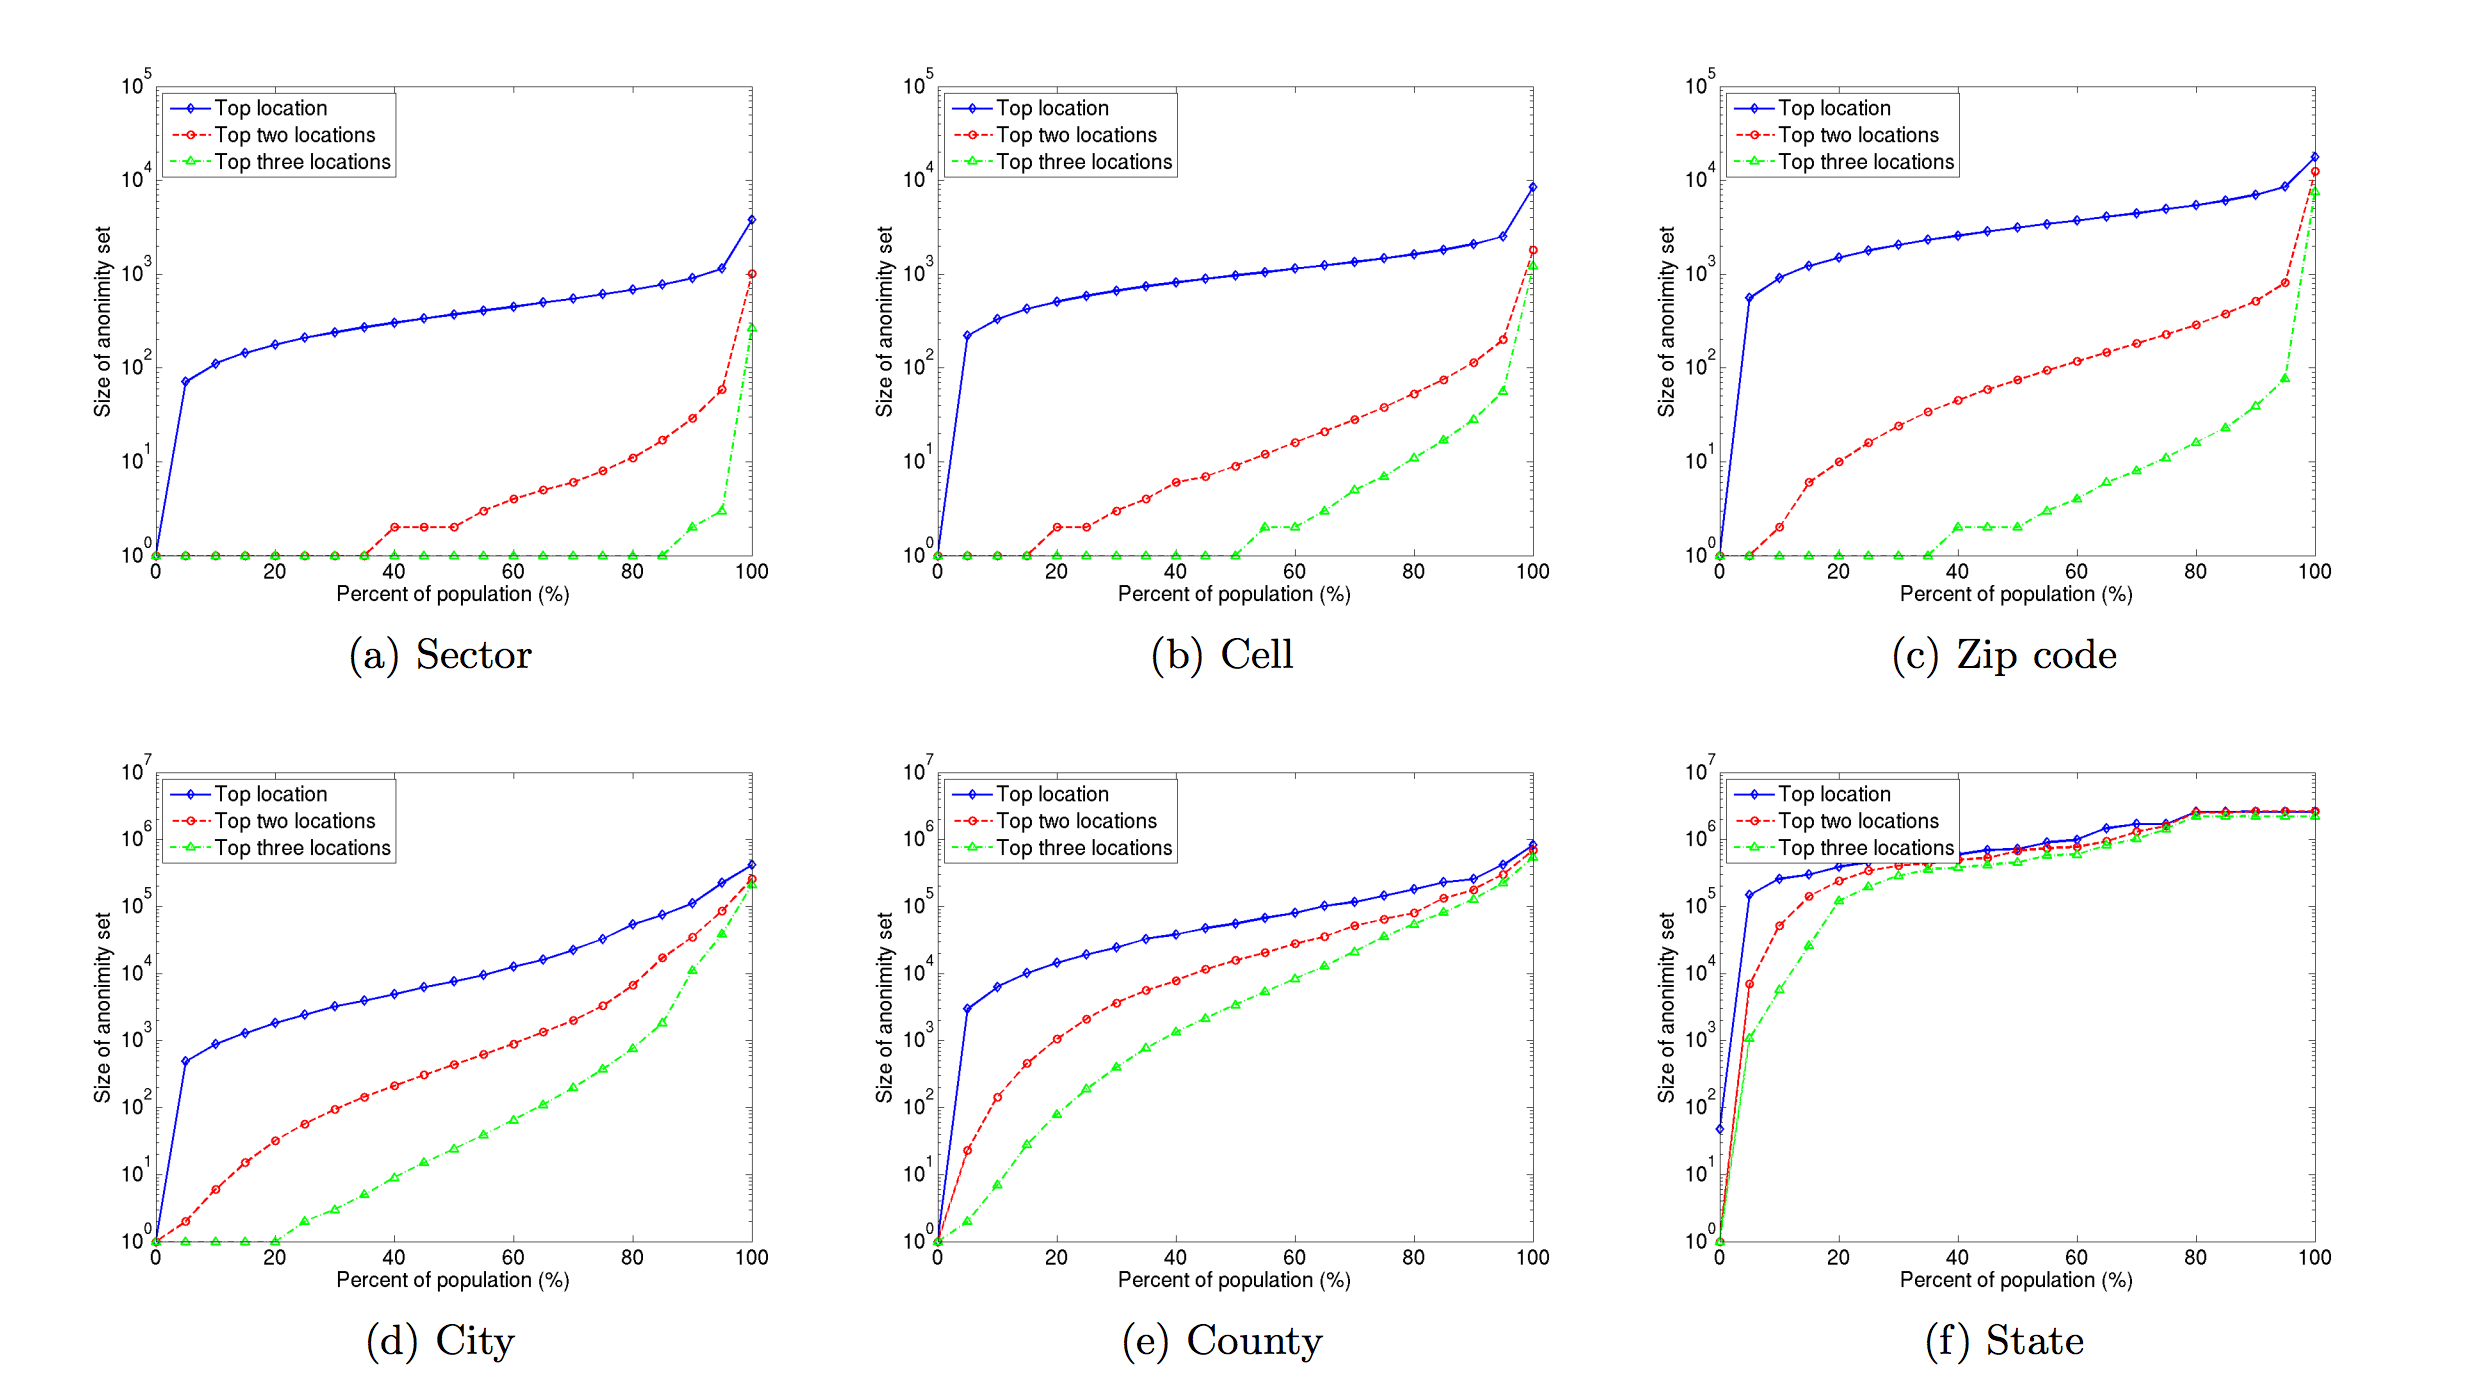
\includegraphics[width=\linewidth]{fig/zang_bolot.png}
  \caption{Figure from~\cite{Zang:2011hk} depicting the size of anonymity sets for top $n$ most visited location of users.
           Locations are varied in granularity, from cell sectors to US states.}
  \label{fig:zang_bolot}
\end{figure}

Location data for individuals is highly unique and thus difficult to anonymize.
The first large-scale study of the $k$-anonymity of location data was appropriately titled ``Anonymization of Location Data Does Not Work"~\cite{Zang:2011hk}.
The paper used data from cell phone call detail records (or CDR, see~\chap{sec:background}) for 25 million United States users over a 3 month period.
The authors represents each user as simply their top $n$ most visited locations, varying $n$ from 1 to 3.
Additionally, the authors varied the granularity of the locations, with the smallest as cell sector and the largest as state.
Remarkably, using 3 locations at a cell level made half of all users completely unique, and 3 locations a sector level made 85\% of all users unique.
A figure detailing this result and results for other granularities and values of $n$ is depicted in~\fig{fig:zang_bolot}.
The authors went on to analyze the impact of geography (comparing different states and cities), mobility (distances between top locations), and social networks on anonymity.


The Montjoye nature report


\subsection{Completed Work}
% Completed work introduction
I have investigated the anonymity of location data for users

\subsubsection{Linking Users Across Domains with Location Data}
% Background...
Although prior work showed location to be highly \emph{unique} and thus posibly \emph{vulnerable} to de-anonymization, no data was actually de-anonymized in practice.
Indeed, just because a data source is highly unique does not mean it can be de-anonymized.
For example, much of cryptography relies on creating highly unique but unpredictable sequences of numbers.
To put it more concretely, imagine that each individual had a die with 1000 sides, and each side represented a location.
If, quite hypothetically, humans decided where to go next by rolling this die, their movements would look very unique.
However, since the movements are random and unpredictable, my movements from different time periods will be indistinguishable from those of a different individual.

TODO: put some math here?

Another possibile break in the argument that uniqueness implies vulnerability is the important factor of sampling.
The datasets dealt with here (phone records, social media posts) are all \emph{actively} collected: each data point exists if and only if the user has taken an action.
Intuitively, the location data from different sampling data sources should look very different.
An individual may be more likely to make phone calls in quiet places, like the home or office, and take geotagged location photos in popular tourist destinations or restaurants.

TODO: put some math here?

In ``Linking Users Across Domains with Location Data", published at WWW in 2016, we tackled this problem, linking users across two entirely different datasets.

% Describe problem setting
\begin{figure*}[t]
  \begin{center}
    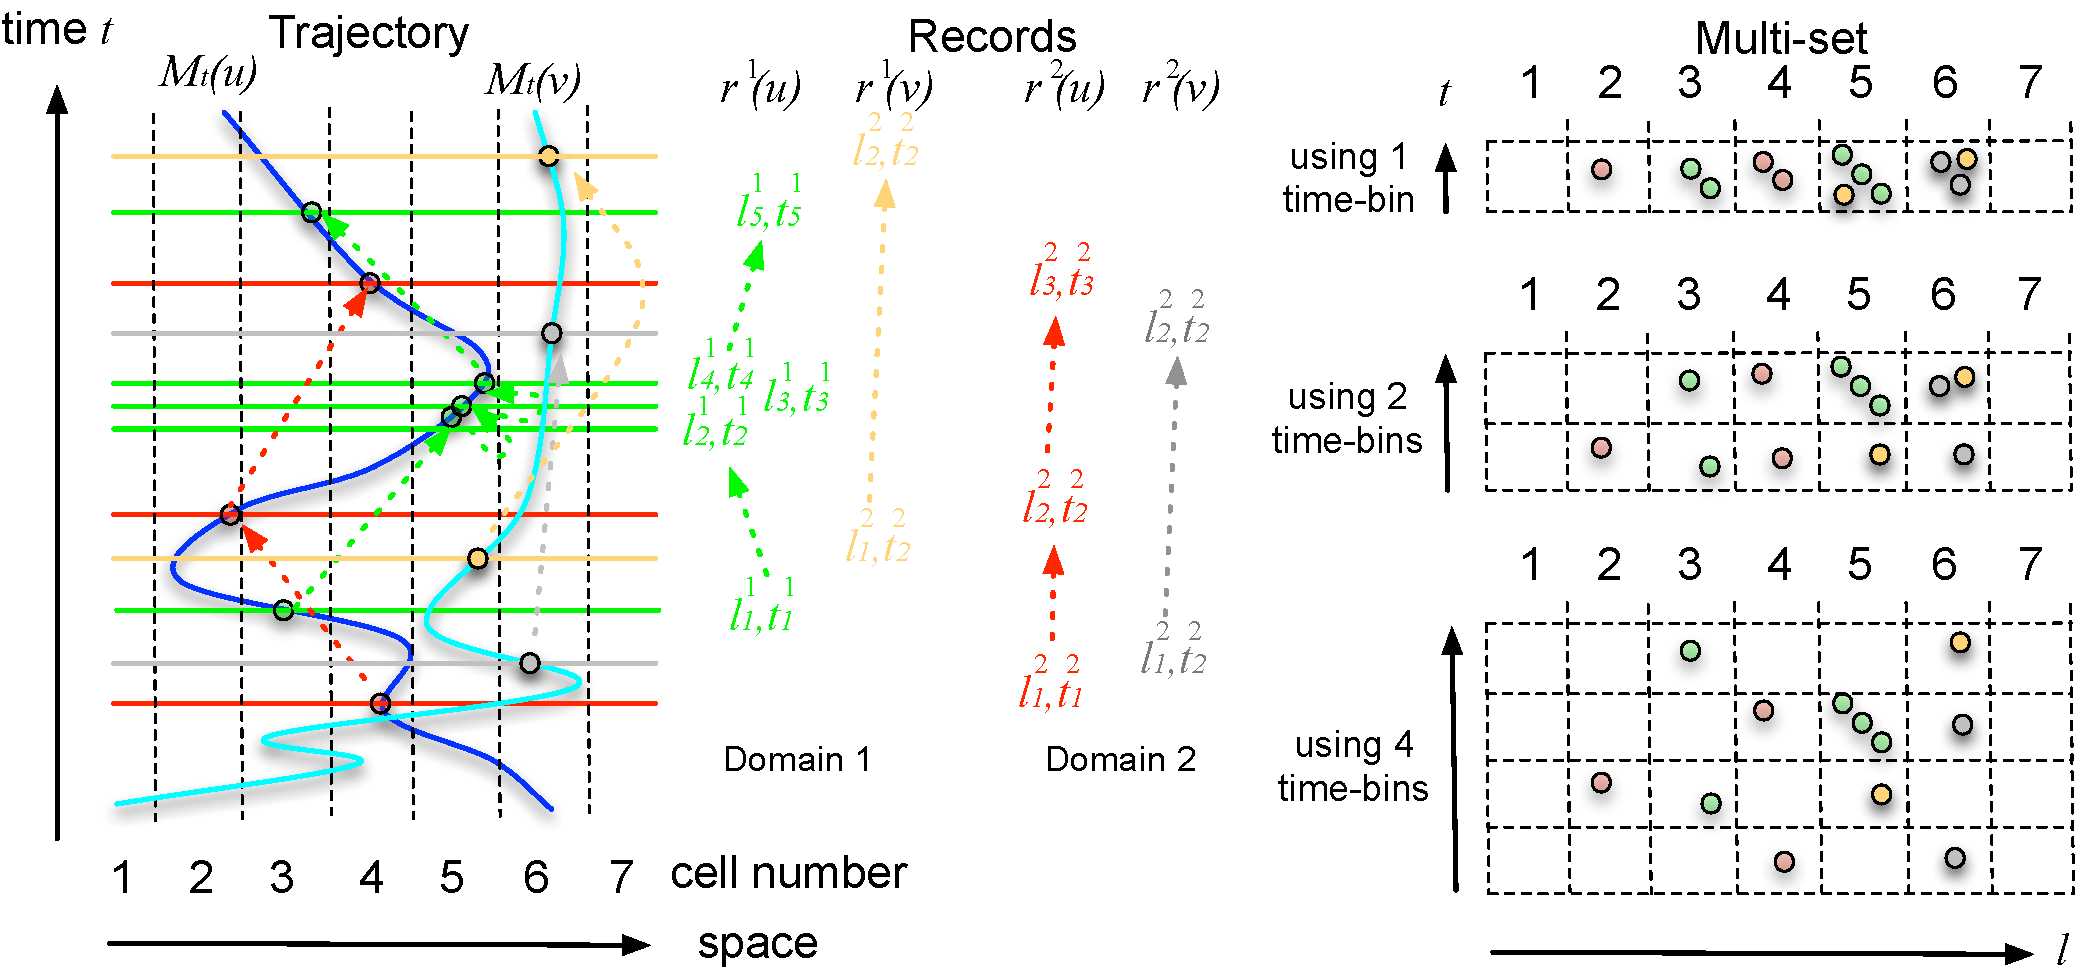
\includegraphics[width=0.65\linewidth]{fig/linking_explain.pdf}
  \end{center}
  \caption{Two space-time trajectories with associated footprints in two domains.}
  \label{fig:linking_explain}
\end{figure*}

% Describe algorithm (and possibly the score)


% Describe dataset

\begin{table*}
  \centering
  \begin{tabular}{llrrrrr}
    % \toprule
            &        & Number & Number  &   Median  &  Number   &           \\
    Dataset & Domain & Users & Checkins &  Checkins & Locations & Date Range\\
    \midrule
    FSQ-TWT   & Foursquare  & 862 & 13,177  & 8    & 11,265 & 2006-10 -- 2012-11 \\
              & Twitter     & 862 & 174,618 & 60.5 & 75,005 & 2008-10 -- 2012-11 \\
    \addlinespace
    IG-TWT    & Instagram   & 1717 & 337,934 & 93 & 177,430 & 2010-10 -- 2013-09 \\
              & Twitter     & 1717 & 447,366 & 89 & 182,409 & 2010-09 -- 2015-04 \\
    \addlinespace
    Call-Bank & Phone Calls       & 452 & $\sim$200k & $\sim$550 & $\sim$3500 & 2013-04 -- 2013-07 \\
              & Card Transactions & 452 & $\sim$40k & $\sim$60 & $\sim$3500 & 2013-04 -- 2013-07 \\
    % \bottomrule
  \end{tabular}
  \caption{Overview of datasets used in study. For FSQ-TWT and IG-TWT, number of locations refers to locations at a 4 decimal GPS granularity (position within roughly 10m).}
  \label{tab:link-data}
\end{table*}

We evaluated this algorithm on multiple real-world datasets.
Gathering the data in itself was a significant challenge, as each dataset needed to contain individuals with identities linked across two different data sources.
Collecting information from one data source is enough of a challenge by itself, given unexpected and changing data formats, connectivity problems, rate limits, and more.
Getting ground truth data across two datasets is thus more difficult, as two APIs need to be dealt with and user identities must be verified across the two.

We gathered three datasets:
\begin{itemize}
  % Data from foursquare checkins and geolocated tweets, from another paper.
  \item \textbf{Foursquare-Twitter} (FSQ-TWT): 
  checkin data from the location-based social networking and review site Foursquare \footnote{\url{https://foursquare.com/}} and geotagged updates from the microblogging site Twitter \footnote{\url{twitter.com}}. 
  This data was obtained in a prior work by other authors who allowed us to use their data~\cite{Zhang:2014ij}.
  We expect the behavior to be somewhat different across the two networks; Foursquare is primarily used to review restaurants, and Twitter is generally used.

  % Geolocated photos and geolocated tweets. Not the exact same. Got twitter account from profile. Medium difficulty.
  \item \textbf{Instagram-Twitter} (IG-TWT):
  Geolocated photographs from the image sharing site Instagram \footnote{\url{instagram.com}} and geotagged updates from the microblogging site Twitter.
  We first crawled Instagram, and then found users who had posted their Twitter usernames in their profiles.
  For each of these users, we used Twitter's API to crawl their public tweets.
  We expected this dataset to be the easiest to link, as there were high numbers of checkins on both sites for most users.

  % Cell phone calls (located to cell tower) and geocoded businesses.
  \item \textbf{Cell phone-Credit Card} (Call-Bank):
  Phone calls associated with geolocated cell towers (CDR) and credit or debit card transaction data associated with geocoded businesses, all from one G20 country.
  Locations were declared the same if the lat-lon of business was within a cell created via a Voronoi tesselation.
  This data was very sparse and the behaviors generating data seems to be very different in the two sets, making us hypothesize that we would have our worst results on it.
\end{itemize}

Statistics about these datasets is summarized in Table~\ref{tab:link-data}.

% Describe results


\subsubsection{FindYou: A Personal Location Privacy Auditing Tool}
